\section{Preprocessing}
\label{sec:preprocess}
For preprocessing, we apply Windowing technique  \cite{windowingct17yahya} with different levels and widths to target specific parts of human organs. Windowing, also known as grey-level mapping, contrast stretching, histogram modification or contrast enhancement is the process in which the CT image grayscale component of an image is manipulated via the CT numbers; doing this will change the appearance of the picture to highlight particular structures. The brightness of the image is adjusted via the window level, window level determines the central or midpoint grey value for the range of HU displayed in the image. Ideal imaging of different tissues depends on the window level. The contrast is adjusted via the window width. A wide window (400-2000 HU) is suitable for examining structures of vastly different attenuation values. For instance, chest structures are best viewed using a wide window.

In or experiments, we apply 3 wide windows corresponding with 3 different versions of a single slice by highlight the abdomen, chest, and spine groups and stack it to one as a three-channel image (Fig. \ref{fig:windowingct}). The window parameters in our experiments are shown in table \ref{table:window_params}
\begin{table}[]
\centering
\caption{Window parameters}\label{table:window_params}
\begin{tabular}{| l | c c |}
\hline
Group      & Window level & Window width \\ \hline
Spine-bone & 900          & 1400         \\ \hline
Tissues    & 200          & 350          \\ \hline
Chest      & 787          & 2137         \\ \hline
\end{tabular}
\end{table}

Where the group of the soft tissue masses can be determined by merging of the abdomen soft tissues and liver. The chest group, which consists of the lungs and mediastinum. By re-calculating the window information from the min value and max value of selected range, these window parameters can be accurately determined.

\begin{figure}[!h]
    \centering
    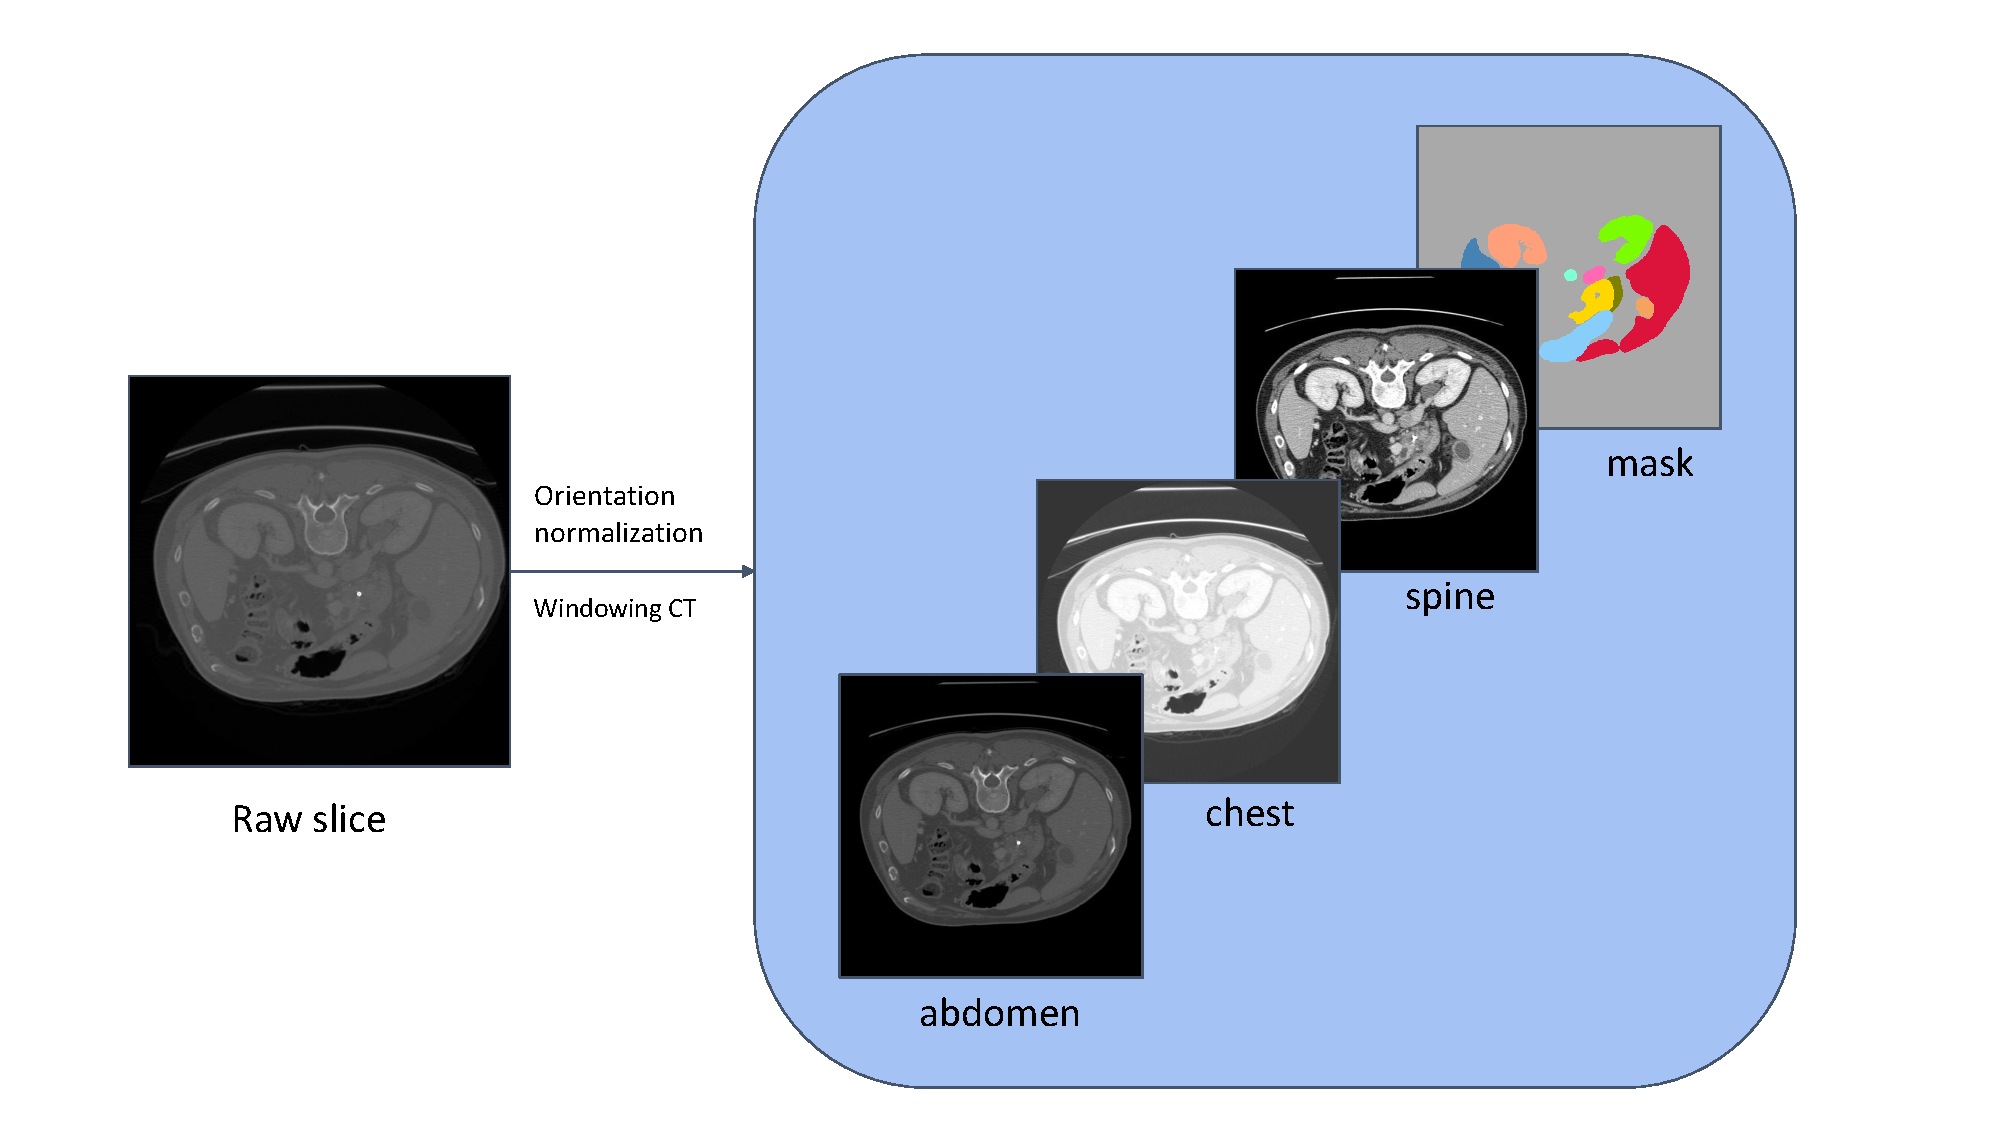
\includegraphics[width=\textwidth]{resources/new_images/preproc.pdf}
    \caption{Windowing CT. 3 different versions are generated from an original slice. }
    \label{fig:windowingct}
\end{figure}

In addition, we choose the axial plane to cut the slices from the CT volumes since this plane has various dimension sizes. 
Due to some relatively small organs, it might be better to keep the original size of the slices without any cropping, resampling, or resizing methods.
The image is rotated to a predefined angle, then divided by 255 for normalization before going through the next step.
\pagebreak